% !TeX program = xelatex
\documentclass[a4paper,12pt]{article}
\usepackage{fontspec} % Для использования системных шрифтов
\usepackage{polyglossia} % Для многоязыковой поддержки
\usepackage{amsmath}

\setmainlanguage{ukrainian} % Основной язык документа
\setotherlanguage{english} % Дополнительный язык документа
\setmainfont{Times New Roman} % Установка шрифта Times New Roman
\usepackage{geometry} % Пакет для настройки полей страницы
\geometry{
	left=3cm,
	right=1.5cm,
	top=2cm,
	bottom=2cm
}

\usepackage{titlesec} % Пакет для настройки заголовков
\titleformat{\section}{\large\bfseries}{\thesection}{1em}{}
\titleformat{\subsection}{\normalsize\bfseries}{\thesubsection}{1em}{}

\usepackage{setspace} % Пакет для настройки межстрочного интервала
\onehalfspacing % Установка полуторного интервала

\usepackage{tocloft} % Пакет для настройки оглавления
\renewcommand{\cftsecleader}{\cftdotfill{\cftdotsep}} % Добавление точек к оглавлению

\usepackage{fancyhdr} % Пакет для настройки колонтитулов
\pagestyle{fancy}
\fancyhf{}
\fancyfoot[C]{\thepage}

\usepackage{hyperref} % Пакет для создания кликабельных ссылок
\usepackage{graphicx}
\usepackage{caption} % Пакет для підписів до зображень


\begin{document}
	
	% Титульная страница
	\begin{titlepage}
		\centering
		\vspace*{1cm}
		
		\huge\textbf{Прямокутник
			найбільшої площі
			вписаний в опуклу
			оболонку}
		
		\vspace{1.5cm}
		
		\raggedleft
		\large
		\begin{tabular}{r}
			\textbf{Лабораторна робота} \\
			Студента 3 року навчання \\
			Групи МІ-31 \\
			Гришечкіна Тихона Сергійовича \\
		\end{tabular}
		
		\vfill
		
		\centering
		\large
		Київ, 2024
		
	\end{titlepage}
	
	% Оглавление
	\tableofcontents
	\newpage
	
	% Анотація українською
	\section*{Анотація}
	У лабораторній було досліджено проблему знаходження прямокутника найбільшої площі, вписаного в опуклу оболонку. Був наведений опис алгоритму, запропонований Бехрузі у 2019 \cite{example1}, а також виконано приклад реалізації алгоритму мовою програмування C\#.
	
	% Анотація англійською
	\section*{Annotation}
	The problem of finding a rectangle of the largest area inscribed in a convex hull was studied in the lab. An algorithm proposed by Behrouzi in 2019 is described \cite{example1}, and an example of the algorithm implementation in the C\# programming language is given.
	\newpage
	
	% Вступ
	\section{Вступ}
		
		Задача пошуку найбільшого вписаного прямокутника є важливою задачею у багатьох галузях, таких як комп'ютерна графіка, робототехніка та обробка зображень. Проблема знаходження найбільшого вписаного прямокутника (НВП) добре досліджена багатьма науковцями. В цілому зазвичай виділяють дві задачі знаходження НВП: задача знаходження НВП зі сторонами паралельними осям координат та загальна.
		
		Наприклад, у праці Деніелса, Міленковича та Рота \cite{example2} досліджено методи та алгоритми для прямокутників зі сторонами паралельними осям координат для різних типів многокутників. А в праці Альта \cite{example3} описано алгоритм для цієї ж задачі у випадку опуклого многокутника «методом дотичних» зі складністю $O(\log(n))$. Це є найкращим результатом для випадку опуклого многокутника, який цікавить нас в рамках цієї лабораторної, що я знайшов у відкритому доступі.
		
		В цій лабораторній буде описано і реалізовано алгоритм Бехрузі \cite{example1} для знаходження НВП зі сторонами паралельними осям координат у випадку опуклого многокутника, що має складність $O(n)$. Але важливо зазначити, що у статті Бехрузі показано, що можна перейти до алгоритму знаходження загального НВП у випадку опуклого многокутника (без обмеження на паралельність осям координат), зі складністю $O(\frac{n}{\epsilon})$, де $\epsilon$ - відносна похибка площі отриманого прямокутника від оптимального.
		
		Важливо зазначити, що хоч і в рамках цієї лабораторної потрібне знаходження опуклої оболонки, \cite{example4} алгоритми її знаходження розглядатися не будуть, а у реалізації буде використано «алгоритм Грехема».
		\begin{figure}[htbp]
			\centering
			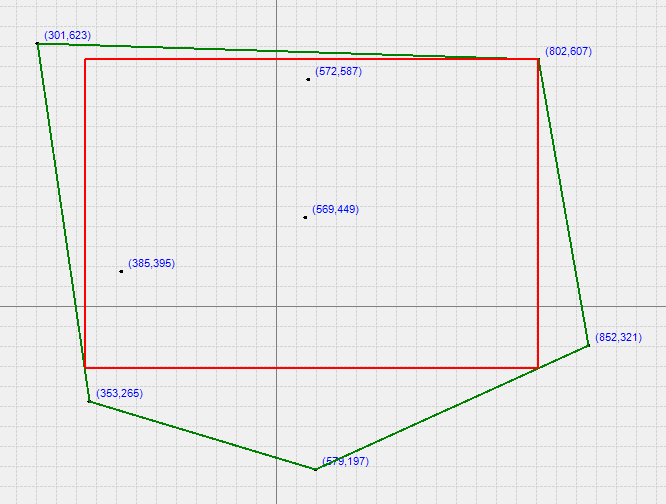
\includegraphics[width=0.6\linewidth]{images/example1}
			\caption{Приклад опуклої оболонки множини точок, з вписаним прямокутником найбільшої площі}
			\label{fig:im_example1}
		\end{figure}
	\newpage
	
	% Основна частина
	\section{Основна частина}
	\subsection{Загальні положення}
	Розглянемо довільний опуклий многокутник $F$ розміру $n$. Тоді можемо сформувати критерій належності точки многокутнику $F$, за допомогою системи з $n$ нерівностей. Для цього проведемо через кожні дві сусідні точки многокутника пряму, та обмежимо за допомогою рівняння цієї прямої точки, які попадають у многокутник. Для наочності рисунок[\ref{fig:im_example2}].
	
	    Врешті-решт, будемо мати:
	\begin{equation*}
		\mathbf{P} = \begin{pmatrix}
			a_{11} & a_{12} \\
			a_{21} & a_{22} \\
			\vdots & \vdots \\
			a_{n1} & a_{n2}
		\end{pmatrix},
	\end{equation*}
	де $P$ - матриця розміру $n \times 2$ (коефіцієнти обмежуючих прямих), та вектор
	\begin{equation*}
		\mathbf{b} = \begin{pmatrix}
			b_1 \\
			b_2 \\
			\vdots \\
			b_n
		\end{pmatrix},
	\end{equation*}
	розміру $n$ (обмежуючі коефіцієнти).
	
	Тоді критерієм належності точки $\mathbf{x}$ многокутнику буде нерівність
	\begin{equation*}
		Px \leq b.
	\end{equation*} 
	
	\begin{figure}[htbp]
		\centering
		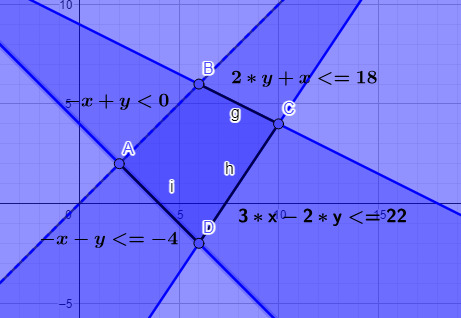
\includegraphics[width=0.6\linewidth]{images/example2}
		\caption{Приклад многукутника $ABCD$, з обмежуючими його нерівностями}
		\label{fig:im_example2}
	\end{figure}
	
	Тепер нехай для довільного багатокутника $F$, маємо довільні три точки $x, y, z$, та вектори $(\vec{u} = y - x, \vec{v} = z - x)$. Рисунок \ref{fig:im_example3} для прикладу.
	Тоді рішенням знаходження найбільшого вписаного прямокутника, буде рішення наступної задачі оптимізації: 
	
	\begin{figure}[htbp]
		\centering
		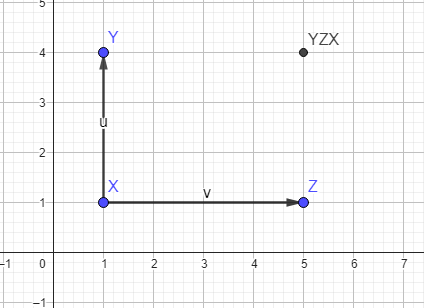
\includegraphics[width=0.6\linewidth]{images/example3}
		\caption{Приклад точок $x,y,z$ та векторів $(\vec{u},\vec{v}	)$}
		\label{fig:im_example3}
	\end{figure}
	
	\begin{equation}
		\max \left| u_1 v_2 - u_2 v_1 \right|
		\label{formula1}
	\end{equation}
	\[
	\text{За умов:}
	\]
	\begin{equation}
		u_1 v_1 + u_2 v_2 = 0
		\label{formula2}
	\end{equation}
	\begin{equation*}
		(x, y, z, y+z-x) \subseteq 
	\end{equation*}
	
	Де формула \ref{formula1}| - максимізація площі шуканих прямокутників. Формула \ref{formula2} - умова ортогональності векторів $u$ та $v$.
	
	\subsection{Опис алгоритму}
	Виходячи з положень, що були описані в попередньому розділі, можемо сформулювати алгоритм для випадку прямокутників зі сторонами паралельними осям координат.

	ауууу


	\subsection{Оцінка складності}
	Тут починається оцінка складності.
	\newpage
	
	% Практична частина
	\section{Практична частина}
	Тут починається практична частина.
	\newpage
	
	% Висновки
	\section{Висновки}
	Тут починаються висновки.
	\newpage
	
	% Додатки
	\section{Додатки}
	Тут починаються додатки.
	\newpage
	
	% Список літератури
	\begin{thebibliography}{9}
		\addcontentsline{toc}{section}{Список літератури} % Добавление списка литературы в оглавление
		\bibitem{example1}
		Behroozi, M. (2019). Largest inscribed rectangles in geometric convex sets. arXiv preprint arXiv:1905.13246.
		
		\bibitem{example2}
		DANIELS, Karen; MILENKOVIC, Victor; ROTH, Dan. Finding the largest area axis-parallel rectangle in a polygon. Computational Geometry, 1997, 7.1-2: 125-148.
		
		\bibitem{example3}
		
		ALT, Helmut; HSU, David; SNOEYINK, Jack. Computing the largest inscribed isothetic rectangle. In: CCCG. 1995. p. 67-72.
		
		\bibitem{example4}
		
		CORMEN, Thomas H., et al. 33.3: Finding the convex hull. Introduction to Algorithms, 1990, 955-956.
	\end{thebibliography}
	
\end{document}
